% !TeX root = ../main.tex
\cleardoublepage
\chapter{数据分析}\label{ch:analysis}

上一章的正式试验(\ref{sec:exp-main}节)中测得了\SIrange{1800}{2600}{\V}电压下的多组数据,并经初步处理得到$F$ -- $p$曲线以及关键点。本章将重点探讨这些数据所揭示出的晶圆脱附的物理过程,并据此判断出数据曲线中的晶圆脱附点,进而得到“脱附背吹压强 -- 电压”数据点。



\section{典型$F$ -- $p$曲线分析}\label{sec:analysis-example}


\subsection{简单型}\label{sec:analysis-example-naive} % 图样图森破,拿衣服

图~\ref{fig:data-fp-2000-4}、图~\ref{fig:data-fp-2000-8}~所示的曲线明显可分为两部分:左下方的部分中,$p$缓慢上升的同时,$F$变化不大;而右方的部分中,$F$随$p$上升而快速上升;两部分中间有明显的转折点。除此转折点以外,可能还有其他的转折点,但对曲线整体走势影响不大。简单型曲线完全符合第\ref{ch:principle}章中对脱附判定的预测,然而实际情况表明,纯粹的简单型曲线占所有检测数据的比例非常小:虽然大部分数据走势与简单型类似,但其组成往往更复杂,在第一次出现$F$随$p$上升而快速上升(走势为向右上方)前后可能存在多个其他类型的转折点;这些特征将在其他曲线类型中介绍,并在\ref{sec:analysis-feature}节中加以分析。

\begin{figure}[tbh]
\centering
\includegraphics
  [max size={0.9\linewidth}{0.9\textheight}]
  {data/fp__2000__4}
\caption{探头受力随背吹压强变化曲线(\SI{2000}{\V} 第4组)}
\label{fig:data-fp-2000-4}
\end{figure}

\begin{figure}[p]
\centering
\includegraphics
  [max size={0.9\linewidth}{0.9\textheight}]
  {data/fp__2000__8}
\caption{探头受力随背吹压强变化曲线(\SI{2000}{\V} 第8组)}
\label{fig:data-fp-2000-8}
\end{figure}


\clearpage


\subsection{回转型}\label{sec:analysis-example-loop}

图~\ref{fig:data-fp-2400-2}、图~\ref{fig:data-fp-2600-2}~所示曲线中能明显观察到一个大回环,其走向为逆时针方向,即:随着试验继续,$p$由逐渐升高转为降低\footnotemark{}的同时,$F$出现一个尖峰,又迅速回落。该特征在很多组数据曲线中均为最明显的特征之一,尤其是在电压较高($V \geq \SI{2200}{\V}$)时。

\footnotetext{此时减压阀开度仍在增加,具体原因在后文中分析。}

\begin{figure}[tbh]
\centering
\includegraphics
  [max size={0.9\linewidth}{0.9\textheight}]
  {data/fp__2400__2}
\caption{探头受力随背吹压强变化曲线(\SI{2400}{\V} 第2组)}
\label{fig:data-fp-2400-2}
\end{figure}

\begin{figure}[p]
\centering
\includegraphics
  [max size={0.9\linewidth}{0.9\textheight}]
  {data/fp__2600__2}
\caption{探头受力随背吹压强变化曲线(\SI{2600}{\V} 第2组)}
\label{fig:data-fp-2600-2}
\end{figure}


\clearpage


\subsection{密集折点型}\label{sec:analysis-example-multi}

观察图~\ref{fig:data-fp-1800-10}、图~\ref{fig:data-fp-2000-7}~所示曲线,发现虽然整体走势与\ref{sec:analysis-example-naive}节中简单型相似,但在两部分曲线中间出现多个相距不远的折点。其他数据曲线中,虽然较少出现与简单型相似的走势,仍有很多具有密集折点特征。

\begin{figure}[tbh]
\centering
\includegraphics
  [max size={0.9\linewidth}{0.9\textheight}]
  {data/fp__1800__10}
\caption{探头受力随背吹压强变化曲线(\SI{1800}{\V} 第10组)}
\label{fig:data-fp-1800-10}
\end{figure}

\begin{figure}[p]
\centering
\includegraphics
  [max size={0.9\linewidth}{0.9\textheight}]
  {data/fp__2000__7}
\caption{探头受力随背吹压强变化曲线(\SI{2000}{\V} 第7组)}
\label{fig:data-fp-2000-7}
\end{figure}


\clearpage


\subsection{倒勾型}\label{sec:analysis-example-sawtooth}

图~\ref{fig:data-fp-2400-6}、图~\ref{fig:data-fp-2600-5}~所示的曲线走势与大部分数据曲线不同:在检测刚开始的时候,$F$即随$p$上升而上升,然后在一点突然出现转折,曲线总体趋势变为$p$上升而$F$反而快速下降。值得注意的是,该类曲线均满足$V \geq \SI{2200}{\V}$。

\begin{figure}[tbh]
\centering
\includegraphics
  [max size={0.9\linewidth}{0.9\textheight}]
  {data/fp__2400__6}
\caption{探头受力随背吹压强变化曲线(\SI{2400}{\V} 第6组)}
\label{fig:data-fp-2400-6}
\end{figure}

\begin{figure}[p]
\centering
\includegraphics
  [max size={0.9\linewidth}{0.9\textheight}]
  {data/fp__2600__5}
\caption{探头受力随背吹压强变化曲线(\SI{2600}{\V} 第5组)}
\label{fig:data-fp-2600-5}
\end{figure}


\clearpage


\subsection{复合型}\label{sec:analysis-example-complex}

正式试验获得的数据中,少数$F$ -- $p$曲线走势较为复杂,包含多种特征,如:图~\ref{fig:data-fp-2200-6}、图~\ref{fig:data-fp-2200-7}~均可视为倒钩型、回转型、简单型的顺序组合;图~\ref{fig:data-fp-2400-7}可视为倒钩型、密集折点型与简单型的顺序组合等等。这类数据揭示了背吹平衡脱附过程本身的复杂性。
%,需通过对其组成特征的分析来加深对其内在物理过程的理解。

\begin{figure}[tbh]
\centering
\includegraphics
  [max size={0.9\linewidth}{0.9\textheight}]
  {data/fp__2200__6}
\caption{探头受力随背吹压强变化曲线(\SI{2200}{\V} 第6组)}
\label{fig:data-fp-2200-6}
\end{figure}

\begin{figure}[tbh]
\centering
\includegraphics
  [max size={0.9\linewidth}{0.9\textheight}]
  {data/fp__2200__7}
\caption{探头受力随背吹压强变化曲线(\SI{2200}{\V} 第7组)}
\label{fig:data-fp-2200-7}
\end{figure}

\begin{figure}[p]
\centering
\includegraphics
  [max size={0.9\linewidth}{0.9\textheight}]
  {data/fp__2400__7}
\caption{探头受力随背吹压强变化曲线(\SI{2400}{\V} 第7组)}
\label{fig:data-fp-2400-7}
\end{figure}



\clearpage



\section{曲线特征与对应物理过程}\label{sec:analysis-feature}

本节将列举一些$F$ -- $p$曲线中较多出现的特征,并结合静电卡盘与检测平台的结构特点,提出关于其对应物理过程的合理猜想。


\subsection{失稳脱附}\label{sec:analysis-feature-destabilize}

当类似\ref{sec:analysis-example-naive}节中图~\ref{fig:data-fp-2000-4}~所示的$p$较小增长引起$F$较大增长的曲线段出现时,一种可能的解释是微力探头与晶圆接触处局部已发生较大尺度的脱附,且静电力与背吹压力构成的平衡不再稳定:随着静电力减小,间隙随之逐渐扩大,引起静电力进一步减小,仅由于晶圆本身刚度以及其他区域吸附力的影响,尚未完全脱附,此时再增加压强,则未能与静电力相平衡的压力将由微力探头对晶圆施加的接触力来平衡,导致$F$迅速随$p$增长。


\subsection{局部脱附 -- 再吸附}\label{sec:analysis-feature-reattach}

图~\ref{fig:data-fp-2000-10-crop}、图~\ref{fig:data-fp-1800-10-crop}~所示的特征在大多数曲线中均有出现,甚至出现多次,且一般为曲线中最早出现的特征。该特征曲线段特点为:折点之前$p$升高而$F$基本不变;当$p$达到一定值时,$F$开始降低,之后$p$也随之降低,直至$F$达到一个新的稳定值;此后$p$回升时,$F$保持新稳定值基本不变。该特征一般在图线中呈现为尺度较小但明显的“乙”或“已”字型。由于试验过程中保证减压阀开度始终单调增加,压强出现下降的原因只能是背吹通道流量增加,说明晶圆与静电卡盘边缘的间隙有所增加;同时,由于微力探头放置在晶圆与卡盘的中心,其受力下降说明晶圆中心处局部与静电卡盘的间隙有所下降。由此推测可能出现的现象是:随着压强增加,晶圆外围出现局部脱附现象(局部失稳),然而并未破坏整体平衡稳定性,之后晶圆在静电力作用下,改变了翘曲模式,进入了能量更低的继续维持稳定吸附的状态。

\begin{figure}[thbp]
\centering
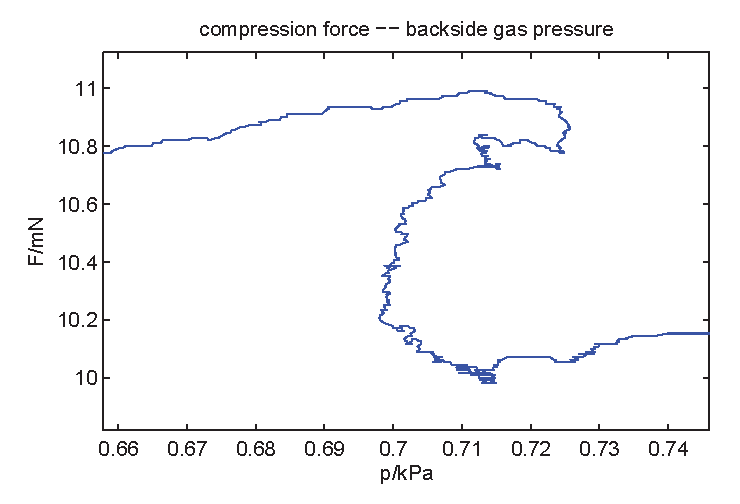
\includegraphics[width=0.8\linewidth]{data/fp__2000__10__crop}
\caption{探头受力随背吹压强变化曲线(\SI{2000}{\V} 第10组\ 局部放大)}
\label{fig:data-fp-2000-10-crop}
\end{figure}

\begin{figure}[thbp]
\centering
\includegraphics[width=0.8\linewidth]{data/fp__1800__10__crop}
\caption{探头受力随背吹压强变化曲线(\SI{1800}{\V} 第10组\ 局部放大)}
\label{fig:data-fp-1800-10-crop}
\end{figure}


\subsection{局部脱附 -- 整体脱附 -- 再吸附}\label{sec:analysis-feature-loop}

以下分析\ref{sec:analysis-example-loop}节所述的“回转”特征:折点之前$p$升高而$F$ 缓慢随之升高;当$p$达到一定值时,$F$突然急剧升高,同时$p$出现明显下降;之后$F$回落,$p$也在下降停止后略微回升,直到$F$达到一个新的稳定值,趋势恢复到与出现折点之前大致相同。采用与\ref{sec:analysis-feature-reattach}节中“乙”字特征相似的分析思路:最初阶段$F$有较为明显的上升,说明晶圆中心处局部间隙在逐步扩大,直至中心失稳脱附,$F$因此急剧升高;但同时在中心的带动下,边缘处间隙也随即扩大,出现整体脱附现象,导致背吹通道流量突增,压强降低,直至不足以与吸附力相平衡,晶圆重新回到稳定吸附状态。

“回转”特征与“乙”字特征的相同之处在于:均出现脱附与再吸附的现象,且再吸附后有可能比脱附前更稳定(静电力更大);不同之处在于:“乙”字特征仅出现局部脱附,而“回转”特征中出现了明显的整体脱附。


\subsection{快速断续脱附}\label{sec:analysis-feature-multi}

\ref{sec:analysis-example-multi}节中描述的“密集折点型”曲线中,有一类包含如图~\ref{fig:data-fp-2000-7}~所示的特征:在较小的压强范围内,交替出现$p$变化不大而$F$向上跳变、$p$上升而$F$基本不变或缓慢上升的两种曲线段,直至$F$跳变越来越大,出现失稳脱附(\ref{sec:analysis-feature-destabilize}节)。与失稳脱附的分析类比,该特征很可能对应晶圆中心局部间隙间断性扩大,逐步失稳并出现整体脱附的物理过程。







%TODO:more features



\section{脱附点的判定}\label{sec:analysis-criterion}

%TODO:criterion




\section{数据汇总与拟合}\label{sec:analysis-tally}

按照上文总结出的数据处理与分析方法,求出正式试验中所有有效数据的脱附压强,并对同电压下的多组数据取中位数\footnotemark{}后,用二次多项式拟合,结果如图~\ref{fig:data-tally},多项式为:
\[
\hat{p} = 0.05919\;\hat{v}^2 + -1.324\;\hat{v} + 1.000
\]
其中,$\hat{p} = p / \SI{1}{\kPa}$,$\hat{v} = v / \SI{1}{\kV}$;拟合相关系数$R^2 = \num{0.9992}$。虽然相关系数较高,说明数据较好地符合拟合多项式,但考虑到在库仑型静电卡盘的静电力理论公式%
(见第\ref{ch:bg}章 \eqref{eq:bg-coulomb}式)%
中,静电力与电压平方成正比,无法解释拟合多项式中的一次项,说明实际静电力产生机理比理论公式复杂,仍有理论公式未能考虑到的因素。

\footnotetext{由于数据点较分散,用中位数能更准确地估计某一电压下的脱附压强真实值。}

\begin{figure}[thbp]
\centering
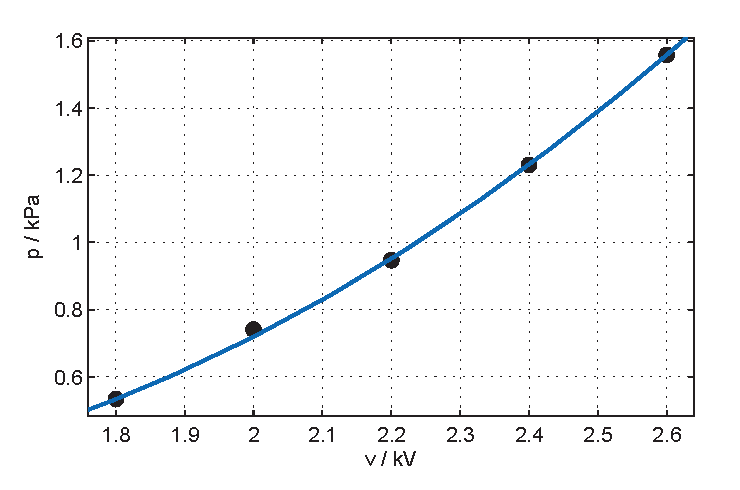
\includegraphics[width=0.8\linewidth]{data/tally}
\caption{脱附背吹压强 -- 电极电压数据点汇总与拟合}
\label{fig:data-tally}
\end{figure}



\section{本章小结}\label{sec:analysis-summary}


